\chapter{Bases de estudio}

\textit{``No esperes a que las condiciones sean perfectas para empezar, es principio hacer las condiciones perfectas.''} 
\textbf{Alan Cohen}
\vspace{1.0cm}

Antes de abordar el estudio de la Física en sí, es necesario entender lo que es la Ciencia y como se genera el conocimiento 
científico.

\section{La Ciencia}

Es un sistema ordenado de conocimientos estructurados que estudia, investiga e interpreta los fenómenos naturales, sociales y 
artificiales. La ciencia  considera y tiene como fundamento las observaciones experimentales.\\ 

Otro concepto de Ciencia es el siguiente:

\begin{tcolorbox}
La Ciencia es el esfuerzo humano concertado para comprender ó comprender mejor la historia del mundo natural y cómo funciona el 
mundo natural, con evidencia física observable como la base de ese entendimiento.
\end{tcolorbox}

En palabras de Brian Greene: ``Para mí, la Ciencia es verdaderamente una forma de vida, una perspectiva, una forma de 
relacionarse 
con el mundo, de tal forma que uno puede emplear un pensamiento racional y una lógica deductiva para entender lo que es 
verdadero, 
lo que es correcto y lo que en verdad es exacto sobre el mundo que nos rodea.''\\
 
Siempre que se genera un conocimiento nuevo o un descubrimiento se dice con certeza que se ha generado Ciencia, y una parte 
fundamental del conocimiento humano es conocer cuales son las leyes fundamentales con las cuales este mundo funciona, y  a eso se 
le llama Ciencia Física, por ello es 
fundamental saber lo que es la Ciencia y el método para generar Ciencia antes de abordar la Física en sí.

\section{El Método Científico:}

Siempre es más saludable comprender las cosas antes que antes que aprenderlas, porque así la generación de la duda y el por qué 
de 
las cosas nos genera la necesidad de saciar nuestras dudas, hallar nuevo conocimiento y hallar una forma correcta de hallarlo. De 
forma general la generación de 
conocimiento nuevo no es el fruto del azar sino más bien del esfuerzo y dedicación humana de manera sistematizada y ordenada 
mediante un proceso definido llamado Método Científico.\\

Este método como su propio nombre indica representa la metodología que define y diferencia el conocimiento de la ciencia de otros 
tipos de conocimientos. Para ello en general el método científico presenta las siguientes etapas para generar conocimiento nuevo:

\subsection{Observación:}
Se trata de la actividad en la cual los sentidos captan a un objeto o aun fenómeno de la realidad y crean la necesidad de 
estudiar 
aquella realidad observada.

\subsection{Inducción:}

En esta etapa se extrae de manera empírica un principio fundamental de la observación mencionada anteriormente.

\subsection{Hipótesis:}

En esta actividad se elabora una explicación a priori de las observaciones o experiencias y las causas posibles.

\subsection{Demostración o experimentación:}

Esta etapa es vital en la generación del conocimiento científico por cuanto en está etapa mediante la experimentación se 
reproduce 
la realidad estudiada bajo el control y medición de los parámetros que intervienen en el mismo, que posteriormente se los analiza 
mediante la estadística y cálculos 
matemáticos se puede llegar a conocer como estos parámetros se comportan durante ese fenómeno estudiado.

\subsection{Demostración o refutación de la Hipótesis:}

En este punto dado el análisis previo se puede relacionarlo con la hipótesis planteada y ver si se cumple o si es falsa.

\subsection{Tesis o teoría científica:}

Este punto es en cual el científico tiene el análisis y observaciones suficientes para llegar a conclusiones y establecimientos 
de 
verdades reproducibles y refutables las cuales ya pueden ser consideradas como conocimiento nuevo. 

\section{Notación científica:}

En ciencias exactas y experimentales muchas de las cantidades que se manejan o son o muy grandes o muy pequeñas que 
necesitan ser representadas de tal manera que no se tenga que escribir demasiados ceros, por ejemplo; resulta molesto escribir un 
número como 0.00000000000000034 varias veces de esa manera, o por ejemplo el número 2440000000000000000000000, y para ello usamos 
las matemáticas de los exponentes, de 
la siguiente manera:

\begin{tcolorbox}
\textbf{Formato de la Notación Científica}\\

La forma general de un número en notación científica es: $a\times 10^n$ donde $1<a<9$ y $n$ es un entero.\\
\end{tcolorbox}


De ese modo se debe poner mucha atención a ese formato para escribir cualquier número correctamente en notación científica.\\

Por ejemplo el número 0.00000000000000034 expresado en notación científica es $3.4\times10^{16}$, y el número 
2440000000000000000000000 en cambio expresado de esta manera es $2.4\times10^{24}$, lo cual se ve que resulta fácilmente más 
comodo usar esta notación y por lo cual demasiado espacio del 
papel.\\

Otros ejemplos:\\

\textit{Números grandes:}\\

$1230,99 = 1,23099\times10^3$\\
$3450000000 = 3,45\times10^{9}$\\
$560000000000000000 = 5,6\times10^{17}$ 

\begin{tcolorbox}
Si se trata de un número grande al cual se quiere expresarlo en notación científica el procedimiento es mover el punto décimal 
hacia la izquierda contando las posiciones que recorre hasta antes el primer dígito de la izquierda y entonces multiplicar este 
número por una potencia de 10 elevado al 
número de posiciones recorridas. 
\end{tcolorbox}

\textit{Números pequeños:}\\

$0,00000045 = 4,5\times10^{-7}$\\
$0,00000006589 = 6,589\times10^{-8}$\\
$0,0000000000000000000000345 = 3,45\times10^{-23}$\\

\begin{tcolorbox}
Si se trata de un número menor que 1 al cual se quiere expresarlo en notación científica el procedimiento es mover el punto 
décimal hacia la derecha contando las posiciones que recorre hasta antes del segundo dígito de la derecha y entonces multiplicar 
este número por una potencia de 10 elevado al número de posiciones recorridas con signo negativo. 
\end{tcolorbox}

En el manejo de este tipo de cantidades resulta común la realización de operaciones matemáticas básicas entre ellas, para lo cual 
se plantea a el lector los siguientes problemas de modo que se familiarize con el uso de estas cantidades:

\subsection{Problemas propuestos:}

Exprese las siguientes cantidades en notación científica:

\begin{itemize}
 \item[a.] 120000000
 \item[b.] 0.00045578
 \item[c.] 45560000
 \item[d.] 0.0000004566
 \item[e.] 0.00000003345
 \item[f.] 7459980000000000000000
 \item[g.] 5670000000000000000
 \item[h.] 0.0000000000278
 \item[i.] 780000000000000000
 \item[j.] 5.06004 
 \item[k.] 0.0007456
 \item[l.] 0.0034521
 \item[m.] 0.00000300004454
 \item[n.] 22825323.2309288487
 \item[o.] 0.000000000000000000455
\end{itemize}

Realice las operaciones siguientes y expresar la respuesta en notación científica:

\begin{itemize}
 \item[j.] $(2,5\times10^{9})\times(4\times10^{-6})$
 \item[k.] $1.2\times10^{-7}-4.2\times10^{-5}$ + $30,4\times10^{-4}$
 \item[l.] $(5,5\times10^{14}-35,4\times10^{13})\times 8.9\times10^{-5}$
 \item[m.] $\frac{7,2\times10^{-30}}{0,008\times10^{-24}}$
 \item[n.] $\frac{0,081\times10^{20}}{0,9\times10^{-34}}$
\item[o.]  $\frac{3,2\times10^{23}}{0,004\times10^{16}}$-$\frac{0,45\times10^{-6}}{0,55\times10^{-10}}$
\item[p.] $\frac{0,081\times10^{20}}{0,9\times10^{-34}}\times(2,5\times10^{12})$
\item[q.] $\sqrt{9,8\times10^{-7}+7,5\times10^{-6}+0.52\times 10^{-6}}$
\item[r.] $((0.00005)^3\times (0.003\times 10^{-3})^{-2})^3$
\item[s.] $\sqrt[5]{\frac{(2.00001\times 10^{-4} - 1.00002\times 10^{-4})^{0.01}}{(0.111111-1.2\times 10^{-2})^{1/3}}}$
\item[t.] $\sqrt{2\times 10^{-5}}-\sqrt{5\times 10^{-2}} + \sqrt{2} - \sqrt{5}$
\item[u.] $ (9\times10^{-8})(4\times 10^{13})(0.4\times10^{-3})-(4.2\times 10^7)(0.5\times10^{-6})$
\end{itemize}

\section{Magnitudes y Medidas:}

Aquella necesidad del hombre por analizar e interpretar de manera objetiva su entorno físico concibio la necesidad de medir 
aquellas cosas que sus sentidos perciben de este mundo.

Y a todo ello que el hombre puede medir se lo denomina \textbf{magnitud}. Y a la acción de medir se trata de la comparación de 
dos 
magnitudes de la misma naturaleza, asignandola a una de ellas como patrón de medida, y de esta manera a aquello que es medible se 
le asigna un número y así es susceptible de un análisis posterior.

\subsection{Sistema Internacional de Medidas (SI)}

Es un conjunto de reglas, normas y disposiciones que rigen a nivel mundial para tener uniformidad en la determinación de una 
medida, la cual se fundamenta en siete unidades fundamentales. Constituye el sistema de unidades adoptado por la Undécima 
Conferencia General de Pesos y Medidas celebrada en 1960.\\ 

Este sistema de unidades ha proporcionado a la comunidad científica un sistema de unidades sencillas y la promulgación de un 
sistema de unidades unificado, teniéndose las siguientes características:

\begin{enumerate}

 \item Posee una sola unidad de medida para cada magnitud y es su principal característica.
 
 \item  Sus unidades se basan en fenómenos físicos fundamentales.

 \item Coherencia, existe una relación lógica y matemática entre sus elementos, unidades, símbolos, múltiplos y submúltiplos.
 
 \item Sencillez, a la voz de los cálculos y operaciones es de fácil uso y aprendizaje.
 
 \item Universabilidad, permite cubrir con sus unidades la totalidad de magnitudes que se encuentran en la ciencia y tecnología.
 
\end{enumerate}


\subsection{Tipos de magnitudes:}

Se dividen en:\\

\textbf{Fundamentales:} Son aquellas que no pueden definirse o derivarse de otras magnitudes, sino más bien ya son de por si 
primarias, es decir, no se definen en función de otras magnitudes, y entre ellas por ejemplo son: masa, la longitud, el tiempo, 
la 
temperatura, la intensidad luminosa, la cantidad de sustancia y la intensidad de corriente. Las unidades fundamentales del SI 
son las siguientes:

\subsubsection{Kilogramo}

Masa del prototipo internacional del kilogramo, adoptado por la Conferencia General de Pesas y Medidas y depositado en la Oficina 
Internacional de Pesas y Medidas, en Sèvres, Francia.\\

Este prototipo es un cilindro de 39 mm de altura y 39 mm de diámetro de una aleación 90\% de platino y 10\% de iridio; tiene 
una densidad aproximada de $21 500 kg/m^3$. 

\subsubsection{Metro}

Longitud del trayecto recorrido por la luz en el vacío en un intervalo de tiempo de 1/299 792 458 segundos.

\subsubsection{Segundo}

Duración de 9 192 631 770 periodos de la radiación correspondiente a la transición entre los dos niveles hiperfinos del estado 
fundamental del átomo de cesio 133. 

\subsubsection{Amperio}

Intensidad de una corriente constante que, mantenida en dos conductores paralelos rectilíneos de longitud infinita, de sección 
circular despreciable y situados a una distancia de un metro uno del otro, en el vacío, produciría entre estos conductores una 
fuerza igual a $2 × 10^{−7}$ newton por metro de longitud. 

\subsubsection{Kelvin}

Fracción 1/273.16 de la temperatura termodinámica del punto triple del agua.

\subsubsection{Mol}

Cantidad de sustancia de un sistema que contiene tantas entidades elementales como átomos hay en 0.012 kilogramos de carbono 12.

\subsubsection{Candela}

Intensidad luminosa, en una dirección dada, de una fuente que emite una radiación monocromática de frecuencia $540 \times 1012$ 
hercios y cuya intensidad energética en esa dirección es 1/683 vatios por estereorradián.\\ 

Y así, la comunidad científica se ha puesto de acuerdo para seguir unos mismos entandares y unidades de medidas ya esto se lo 
llama: El Sistema Internacional de Unidades (SI), el cual utiliza por convención siete magnitudes fundamentales: 

\begin{table}[H]
\centering
\begin{tabular}{lccc}
\hline
Magnitud & Unidad de medida & Símbolo & Dimensión\\
\hline
Masa & kilogramo & kg & M\\
Longitud & metro & m & L\\
Tiempo & segundo & s & T\\
Temperatura & kelvin & K & $\Theta$ \\
Intensidad luminosa & candela & cd & $\Psi$\\
Cantidad de sustancia & mol & mol & N\\
Intensidad de corriente & amperio & A & I\\
\hline
\end{tabular}
\caption{Tabla de magnitudes fundamentales.} 
\end{table}

\textbf{Derivadas:} Son aquellas magnitudes que se derivan por la combinación de las magnitudes fundamentales, por ejemplo: el 
área, el volumen, el peso, la energía, la velocidad, etc.\\

Tambíen tenemos otro tipo de magnitudes que son \textbf{complementarias} a las antes ya mencionadas:

\begin{table}[H]
 \begin{center}
 \begin{tabular}{llcc}
 \hline
Magnitud & Unidad de medida & Símbolo & Dimensión\\
\hline
Ángulo plano & radián & rad & $\alpha$ \\
Ángulo sólido & estereoradián & sr & $\omega$ \\
\hline
 \end{tabular}
 \caption{Tabla de magnitudes complementarias.}
 \end{center}
\end{table}

\section{Múltiplos y submúltiplos:}

Para representar las medidas de diferentes magnitudes las cuales presentan cantidades muy grandes o muy pequeñas hace falta 
establecer un estándar de prefijos de múltiplos y submúltiplos de la siguiente manera:

\begin{table}[H]
 \begin{center}
\begin{tabular}{rccc}
\hline
Factor numérico & Exponente & Prefijo & Símbolo\\
\hline
1 000 000 000 000 000 000 000 000 & $10^{24}$ & yotta & Y \\
1 000 000 000 000 000 000 000 & $10^{21}$ & zetta & Z \\
1000 000 000 000 000 000 & $10^{18}$ & exa & E\\
1000 000 000 000 000 & $10^{15}$ & peta & P\\
1000 000 000 000 & $10^{12}$ & tera & T\\
1000 000 000 & $10^{9}$ & giga & G\\
1000 000 & $10^{6}$ & mega  & M\\
1000 &$10^{3}$ & kilo & k\\
100 & $10^{2}$ & hecto & h\\
10 & $10^{1}$  & deca & da\\
\hline
\end{tabular}
\caption{Tabla de múltiplos del SI.}
 \end{center}
\end{table}
 
\begin{table}[H]
 \begin{center}
\begin{tabular}{rccc}
\hline
Factor Numérico & Exponente & Prefijo & Símbolo\\
\hline
0.1 & $10^{-1}$ & deci & d\\
0.01 & $10^{-2}$ & centi & c\\
0.001 & $10^{-3}$ & mili & m\\
0.000001 & $10^{-6}$ & micro & $\mu$\\
0.000000001 & $10^{-9}$ & nano  & n\\
0.000000000001 & $10^{-12}$ & pico & p\\
0.000000000000001 & $10^{-15}$ & femto & f\\
0.000000000000000001 & $10^{-18}$  & atto & a\\
0.000 000 000 000 000 000 001 & $10^{-21}$ & zepto & z\\
0.000 000 000 000 000 000 000 001 & $10^{-24}$ & yocto & y\\
\hline
\end{tabular}
\caption{Tabla de submúltiplos del SI.}
 \end{center}
 \end{table}
 
\subsection{Análisis dimensional}

La palabra dimensión\footnote{Cualquier elemento del conjunto de cantidades o unidades basicas de las cuales se pueden derivar el 
resto, por ejemplo, masa, longitud, tiempo} tiene un significado especial en Física, y por lo general ($[\quad]$) denota la 
naturaleza física de una cantidad. Por ejemplo las distancias pueden medirse en metros.\\

\textbf{Ejemplo:} $[\text{velocidad}] = [v] =\frac{L}{T^2}$, $[\text{área}] = [A] = L^2$\\
 
El análisis dimensional sirve para deducir o verificar la validez de una fórmula específica ó para comprobar su expresión final.\\

\textbf{Ejemplo:} Siendo la fórmula de la velocidad final en un tipo de movimiento la siguiente: $v_f = v_0 + at$, la analizo 
dimensionalmente: $[v_f] = [v_0] + [a][t] = \frac{L}{T} = \frac{L}{T} + \frac{L}{T^2}T$, y por tanto compruebo que tiene validez 
dimensional.

\subsection{Problemas del SI:}

Convertir las siguientes magnitudes a lo que se indica:
\begin{itemize}
 \item[1.] 3 cm a m.
 \item[2.] 3.4 $\mu s$ a minutos.
 \item[3.] 4 kg a gramos.
 \item[4.] 5,1 ns a horas.
 \item[6.] 5 dm a cm.
 \item[7.] 19 mg a kg.
 \item[8.] 43 fs a ns.
 \item[9.] 14 ps a $\mu s$.
 \item[10.] 74 libras a gramos.
 \item[11.] 11 $cm^2$ a $m^2$.
 \item[12.] 6,7 $m^3$ a $cm^3$.
 \item[13.] 0,967 $\mu m^2$ a $mm^3$.
 \item[14.] 54 m/s a km/h.
 \item[15.] 78 km/h a m/s.
 \item[16.] 86 cm/s a m/min.
 \item[17.] 25 km/h a cm/s.
 \item[18.] 32 $kg/m^3$ a $g/cm^3$.
 \item[19.] 92 $m^3/s$ a $cm^3/s$.
 \item[20.] 73 $g/cm^2$ a $kg/m^2$.
 \item[21.] Encuentre el valor de:\\
 $\frac{(0,9997895\times 10^{-7}pm)^2(2,714\times 10^8 ns)}{(1124.45\times 10^{-3} fm)(5,27\times 10^4 Ekg)}\times 
\left(\frac{346512,345\times 10^{-6} \mu kg}{0,00023 Ts}\right)^3$.
 \item[22.] Realice el análisis dimensional del resultado del anterior problema.
\item[23.] Si tuviésemos un terrón en forma de cubo de 8 $m^3$ de volumen y nos disponemos a dividirlo en terrones de 1 $cm$ de 
lado, ¿cuántos terrones obtendríamos?
\item[24.] La edad de la Tierra es aproximadamente 4500 000 000 años. Exprese esta cantidad en segundos y en notación
científica.
\item[25.] La masa de un electrón es $9 \times 10
^{-31}Kg$. Las masas de un
 protón y de un neutrón son $1,6725 \times 10
^{
-27} Kg$ y $1,6748 \times 10
^{-27} Kg$, respectivamente.
 Determine la masa de un átomo de azufre sabiendo que tiene 16 
electrones, 16 protones y
 16 neutrones. Expresa la respuesta en notación científica.

\item[26.] El
 diámetro de un virus es $5 \times 10^{-4} mm$. ¿Cuantos de esos virus son necesarios para rodear
 la Tierra? 
(Radio de la Tierra: 6370 km) 

 \end{itemize}

\section{Fórmulas}

Una fórmula es una expresión matemática de una ley o principio general que hace el uso de números, símbolos y letras. En Física 
las fórmulas indican las relaciones que existen entre varias magnitudes de un mismo fenómeno. Es clave entender el significado 
físico de cada magnitud y el contexto de la aplicación de una fórmula física.\\

Así, por ejemplo en Geometría es conocido que el área de un triángulo es igual a la mitad del producto de la base $b$ por la 
altura $h$ de ese triángulo, es decir: $A = \frac{1}{2}b\times h$.\\

Las fórmulas son usadas en las ciencias como la Matemática, Física, Química, etc, y son de enorme utilidad, ya que expresan de 
manera simplificada una ley o principio general, son fáciles de recordar y su aplicación es fácil.

\subsection{Despeje de fórmulas}

Despejar una variable en una fórmula o ecuación es el proceso que lleva a encontrar una ecuación equivalente en que la variable 
esté aislada en un miembro de la ecuación. Al despejar una variable en una ecuación conseguimos una fórmula en que la variable 
está expresada en términos de las otras variables mediante el uso de las leyes del Algebra de tal modo que consigamos el correcto 
despeje. Cabe mencionar que la dificultad de un despeje en particular depende exclusivamente de la forma de la fórmula.  


\subsubsection{Problemas de despeje de fórmulas:}

En las fórmulas mostradas despejar las magnitudes que se señalan:

\begin{enumerate}
 \item $d$ y $t$ en $v = \frac{d}{t}$.
 \item $v_0$ y $a$ en $v_f = v_0 + at$.
 \item $a$, $v_{0}$ y $t$ en $d = v_{0} t + \frac{1}{2} at^2$.
 \item $a$ en $k = \frac{f - g}{b - a}$.
 \item $b$ en $q = q_0 \sqrt{a-b}$.
 \item $t$ en $\lambda = \lambda_0 e^{-kt}$.
 \item $m$, $g$,$h$ y $v$ en $E = \frac{1}{2}mv^2 + mgh$.
 \item $a$ en $c^2 = a^2 + b^2$.
 \item $c$ en $E = mc^2$.
 \item $B$ en $A = \frac{B + b}{2}$.
 \item $c$ en $A = \sqrt{s(s-a)(s-b)(s-c)}$.
 \item $\alpha$ en $\frac{b}{\sen(\beta)}=\frac{a}{\sen(\alpha)}$.
 \item $m'$ y $r$ en $F = G\frac{mm'}{r^2}$.
 \item $\theta$ en $W = Fd cos(\theta)$.
 \item $w$ en $F = -mw^2r$.
 \item $m_1$ en $x = \frac{m_1x_1+m_2x_2}{m_1+m_2}$.
 \item $d$ y $v_0$ en $v^2 = v_0^2 -2ad$.
 \item $R_2$ en $\frac{1}{R} = \frac{1}{R_1} + \frac{1}{R_2}$.
 \item $k$ y $w$ en $s^m = t_v + \log_{12}(k-w^2)t$.
 \item $p$ y $c$ en $E^2 = m^2 c^4 + p^2c^2$.
 \item $a$ en $r = t +\frac{1}{3}(\frac{a}{x-a})^2$.
 \item $v$ en $m = \frac{m_0}{\sqrt{1-\frac{v^2}{c^2}}}$.
 \item $g$ en $T = 2\pi\sqrt{l/g}$.
 \item $w$ en $A = K cos(ku - wt)$.
 \item $a$ y $c$ en $x = \frac{-b \pm \sqrt{b^2-ac}}{2a}$.
 \item $i$ en $a = 3j - \frac{q}{q-i}$.
 \item $k$ y $\lambda$ en $j = j_0 e^{-\lambda\sqrt{k-k_0}}$.
 \item $u$ y $v$ en $\log_{v}(10) < \log_{u}(kt) - st$.
 \item $\beta$ en $C =  \frac{6\zeta P_0^2 + 3\beta}{4\zeta P_0^2 + 3\beta}$.
 \item $\zeta$ en $\xi = \frac{\sqrt{g}}{P_0\left( \zeta P_0^2+\frac{1}{2}\beta\right)^{1/2}}$.
 \end{enumerate}



\chapter{Cantidades escalares y vectoriales:}

\textit{``Dios algunas veces geometriza''.} \textbf{Platón} 
\vspace{1.00cm}

Cuando alguien empieza sus primeros pasos en la Física se encontrará con dos tipos de cantidades bien definidas como son: las 
cantidades \textbf{escalares} y \textbf{vectoriales}.\\

\section{Escalares}

Las cantidades escalares se definen simplemente por un valor numérico o algún valor numérico con alguna unidad de 
medida. Es decir, se trata de simplemente de un número que puede estar acompañado de alguna unidad de medida. Tambíen 
en la Física se lo conoce a los escalares como tensores de grado cero. Ejemplos: 10 cm, 3, -4,3, 4 kg, 34 km/h, etc.

\section{Vectores}

Las cantidades vectoriales en cambio necesitan para definirsa tres características: módulo, dirección y sentido. 
Gráficamente a las cantidades vectoriales se las representa por medio de una flecha.\\

Los vectores se representan geométricamente con flechas y se le asigna por lo general una letra que en su parte 
superior lleva una pequeña flecha de izquierda a derecha como se muestra en la figura siguiente:\\  

\begin{figure}[H]
   \centering
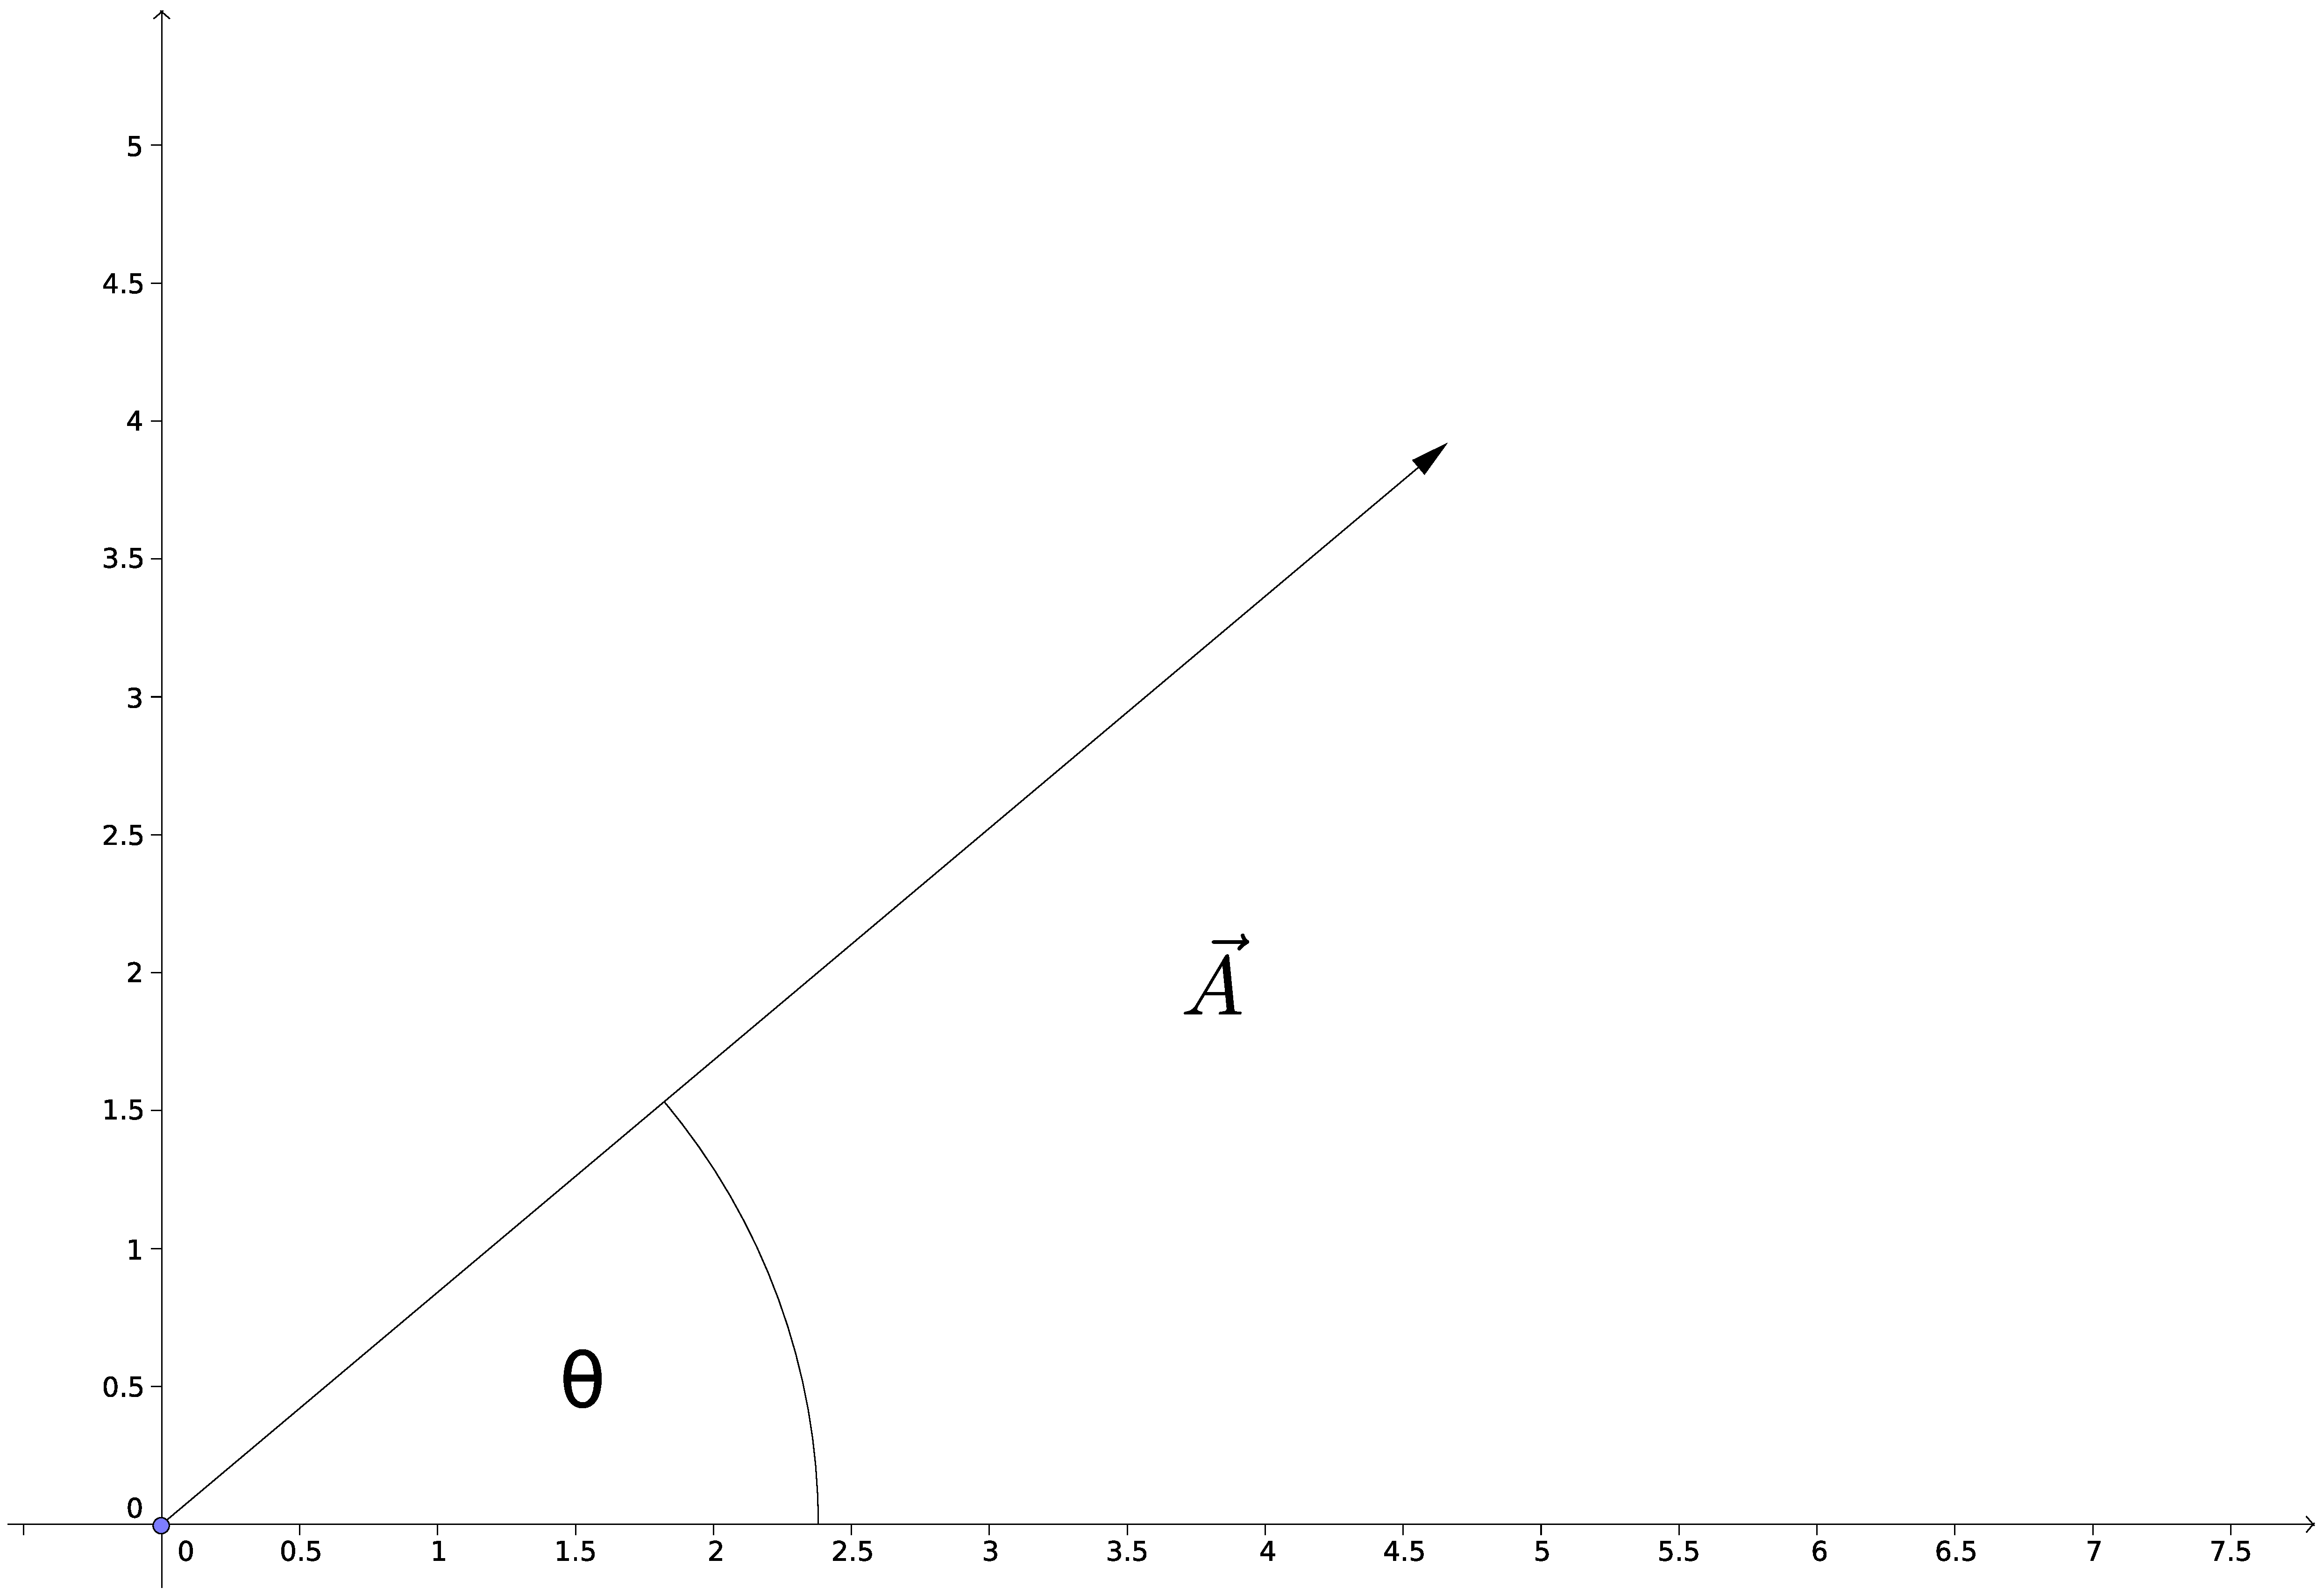
\includegraphics[width=0.7\textwidth]{images/vector_uno.eps}
  \caption{\small{Representación de un vector $\vec{A}$ en el plano cartesiano.}}
   \end{figure}

\textbf{Módulo}\\

El módulo de un vector queda definido como la longitud o tamaño que tiene la flecha que lo representa gráficamente y se 
representa como A, $|\vec{A}|$ ó $\|\vec{A}\|$. También denominado como la intensidad del vector.\\

\textbf{Dirección:}\\

Es el ángulo ($\theta$) que se forma desde la horizontal hasta el vector tomando el sentido antihorario como positivo y negativo 
en el sentido horario.\\

\textbf{Sentido:}\\

El sentido se refiere a la línea acción del vector, ó mejor dicho hacia donde apunta la flecha del vector.\\

Todo vector tiene un vector opuesto que se trata de un vector con el mismo módulo pero con su sentido contrario y se 
simboliza con un signo menos $-\vec{A}$.\\

\subsection{Representación en coordenadas cartesianas:}

\begin{figure}[H]
   \centering
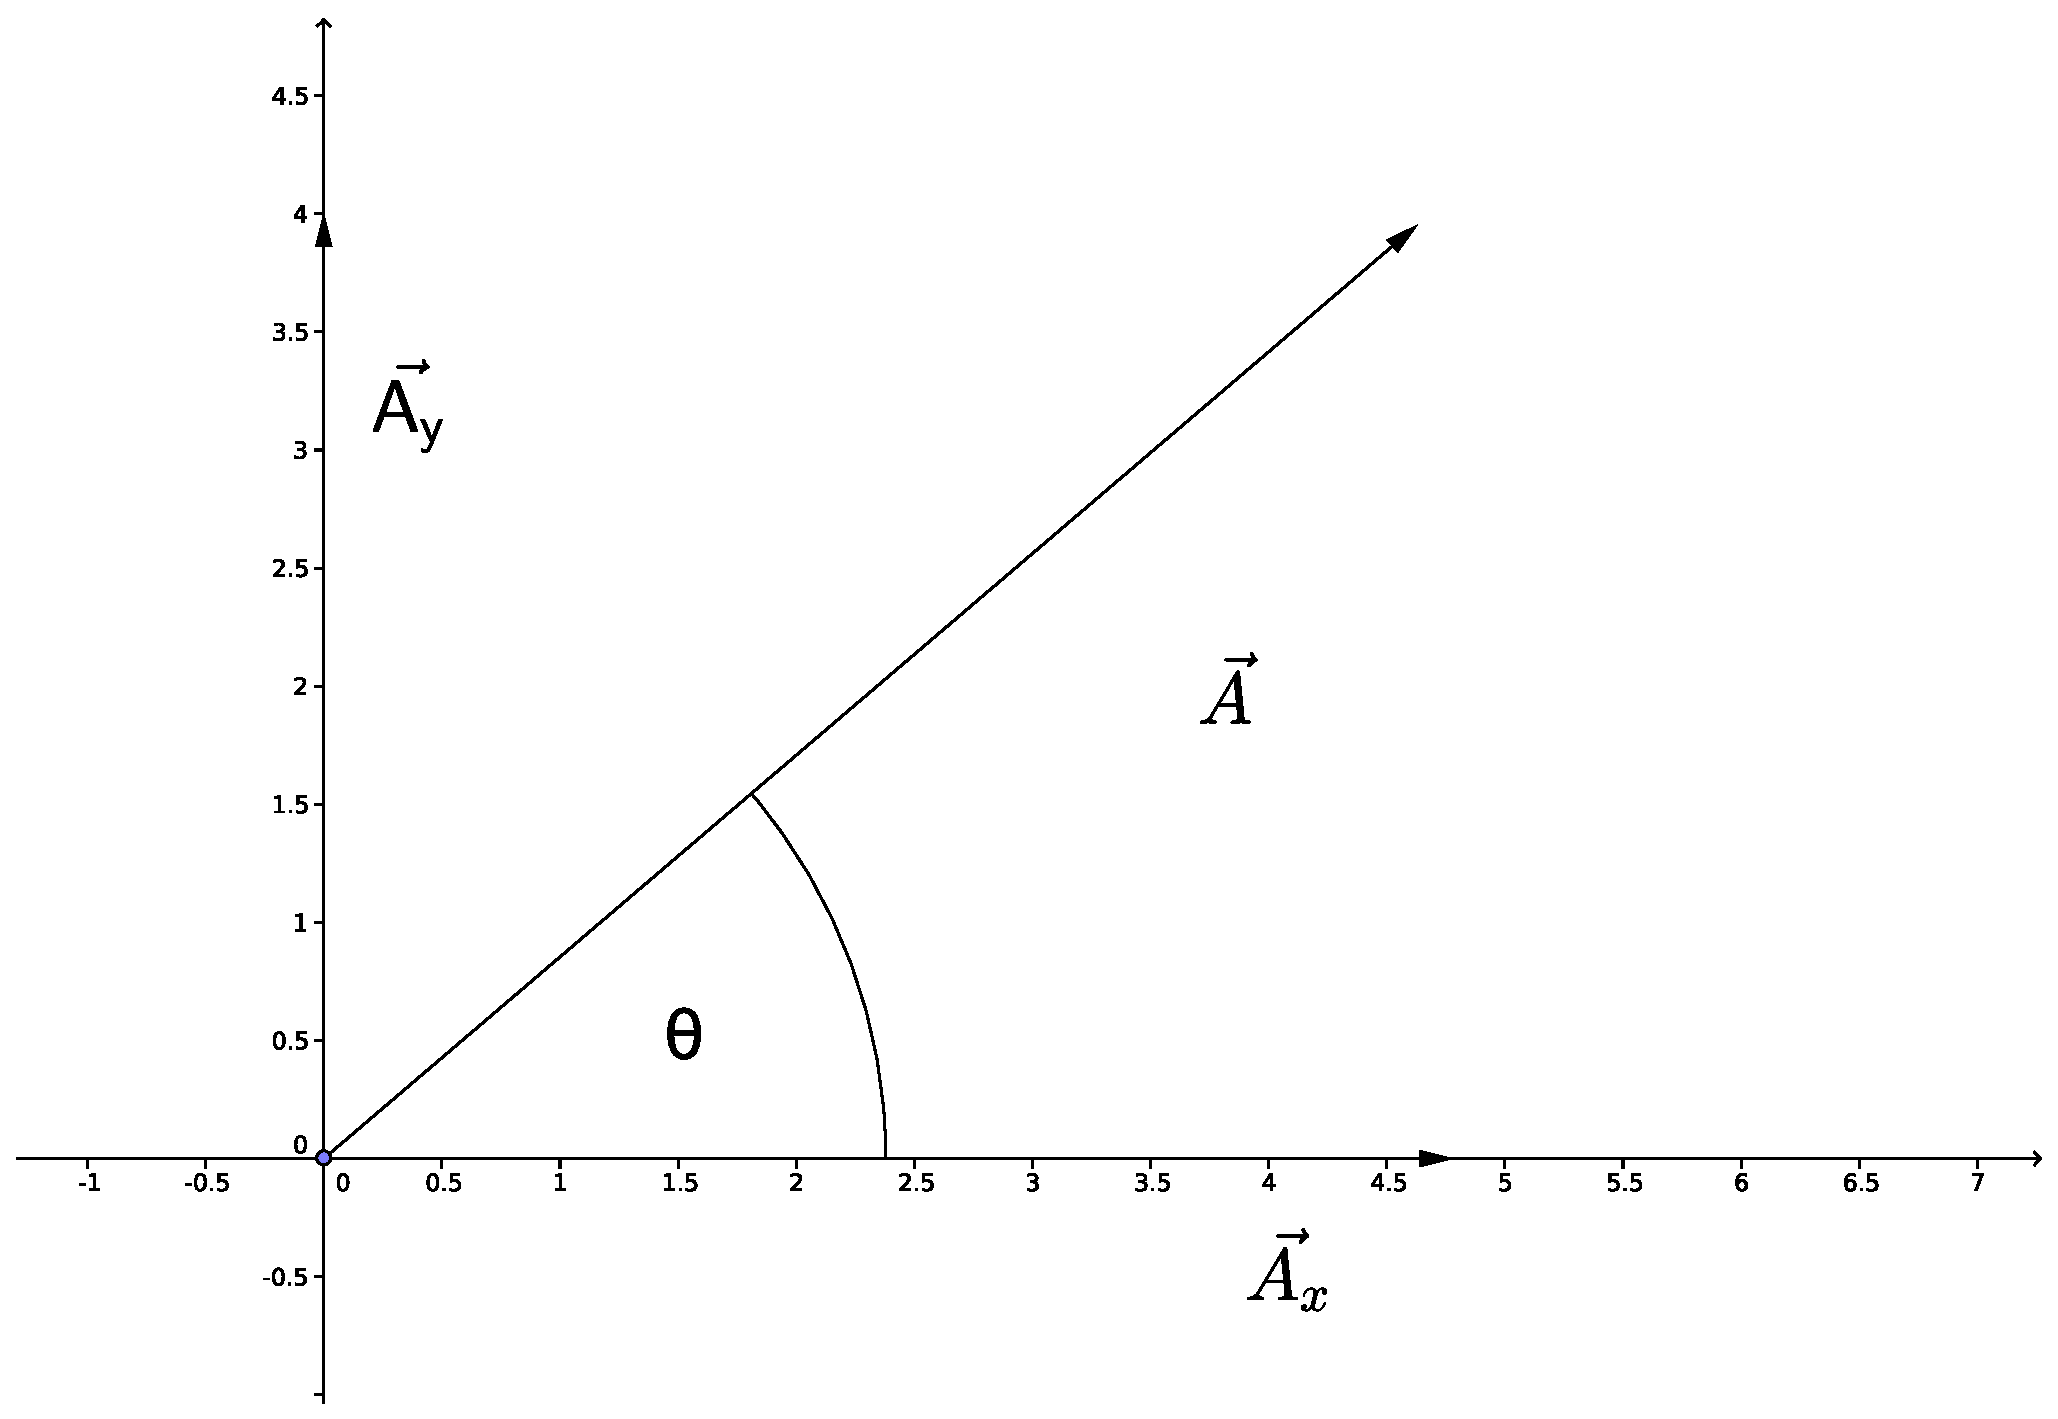
\includegraphics[width=0.7\textwidth]{images/vector_dos.eps}
  \caption{\small{Representación de las coordenadas cartesianas del vector $\vec{A}$ en el plano cartesiano.}}
   \end{figure}

En Matemáticas y Física a los vectores los representamos mediante un sistema de referencia cartesiano, y así de esta 
manera todo vector posee lo que se denomina coordenadas rectángulares. Estas componentes son las proyecciones del 
vector en cada uno de los ejes cartesianos, en otros palabras, son los vectores que se forman al proyectar 
perpendiculares desde el punto extremo del vector hacia los ejes coordenados.\\


Las coordenadas cartesianas o rectángulares de un vector $\vec{A}$, se calcula como:

\begin{equation}
A_x = Acos(\theta) \quad y \quad A_y = Asen(\theta) 
\end{equation}

donde $A_x$ es la componente del vector $\vec{A}$ en el eje de las $x$, y $A_y$ es la componente del mismo vector en el 
eje de las $y$.\\

La dirección del vector se lo encuentra de la siguiente manera:

\begin{equation}
 \theta = tan^{-1}(\frac{A_y}{A_x})
\end{equation}

, y por su puesto el módulo del vector queda definido en función de sus componentes como:

\begin{equation}
 |\vec{A}| = \sqrt{A_x^2 + A_y^2}
\end{equation}

\subsubsection{Ángulos y cosenos directores:}

Son aquello ángulos que parten desde los ejes coordenados positivos hacia el vector y cuyo valor esta en el intervalo 
de $0^\circ$ a $180^\circ$. El que parte desde el eje de las abcisas se simboliza como $\alpha$, mientras que el que 
parte desde el eje de las ordenadas se le simboliza como $\beta$.\\

Y a los cosenos directores son los cosenos de los ángulos directores simplemente:

\begin{equation}
 cos(\alpha) =\frac{A_x}{A}  \quad y \quad cos(\beta)=\frac{A_y}{A}
\end{equation}

\subsection{Representación en coordenadas polares:}

\begin{figure}[H]
   \centering
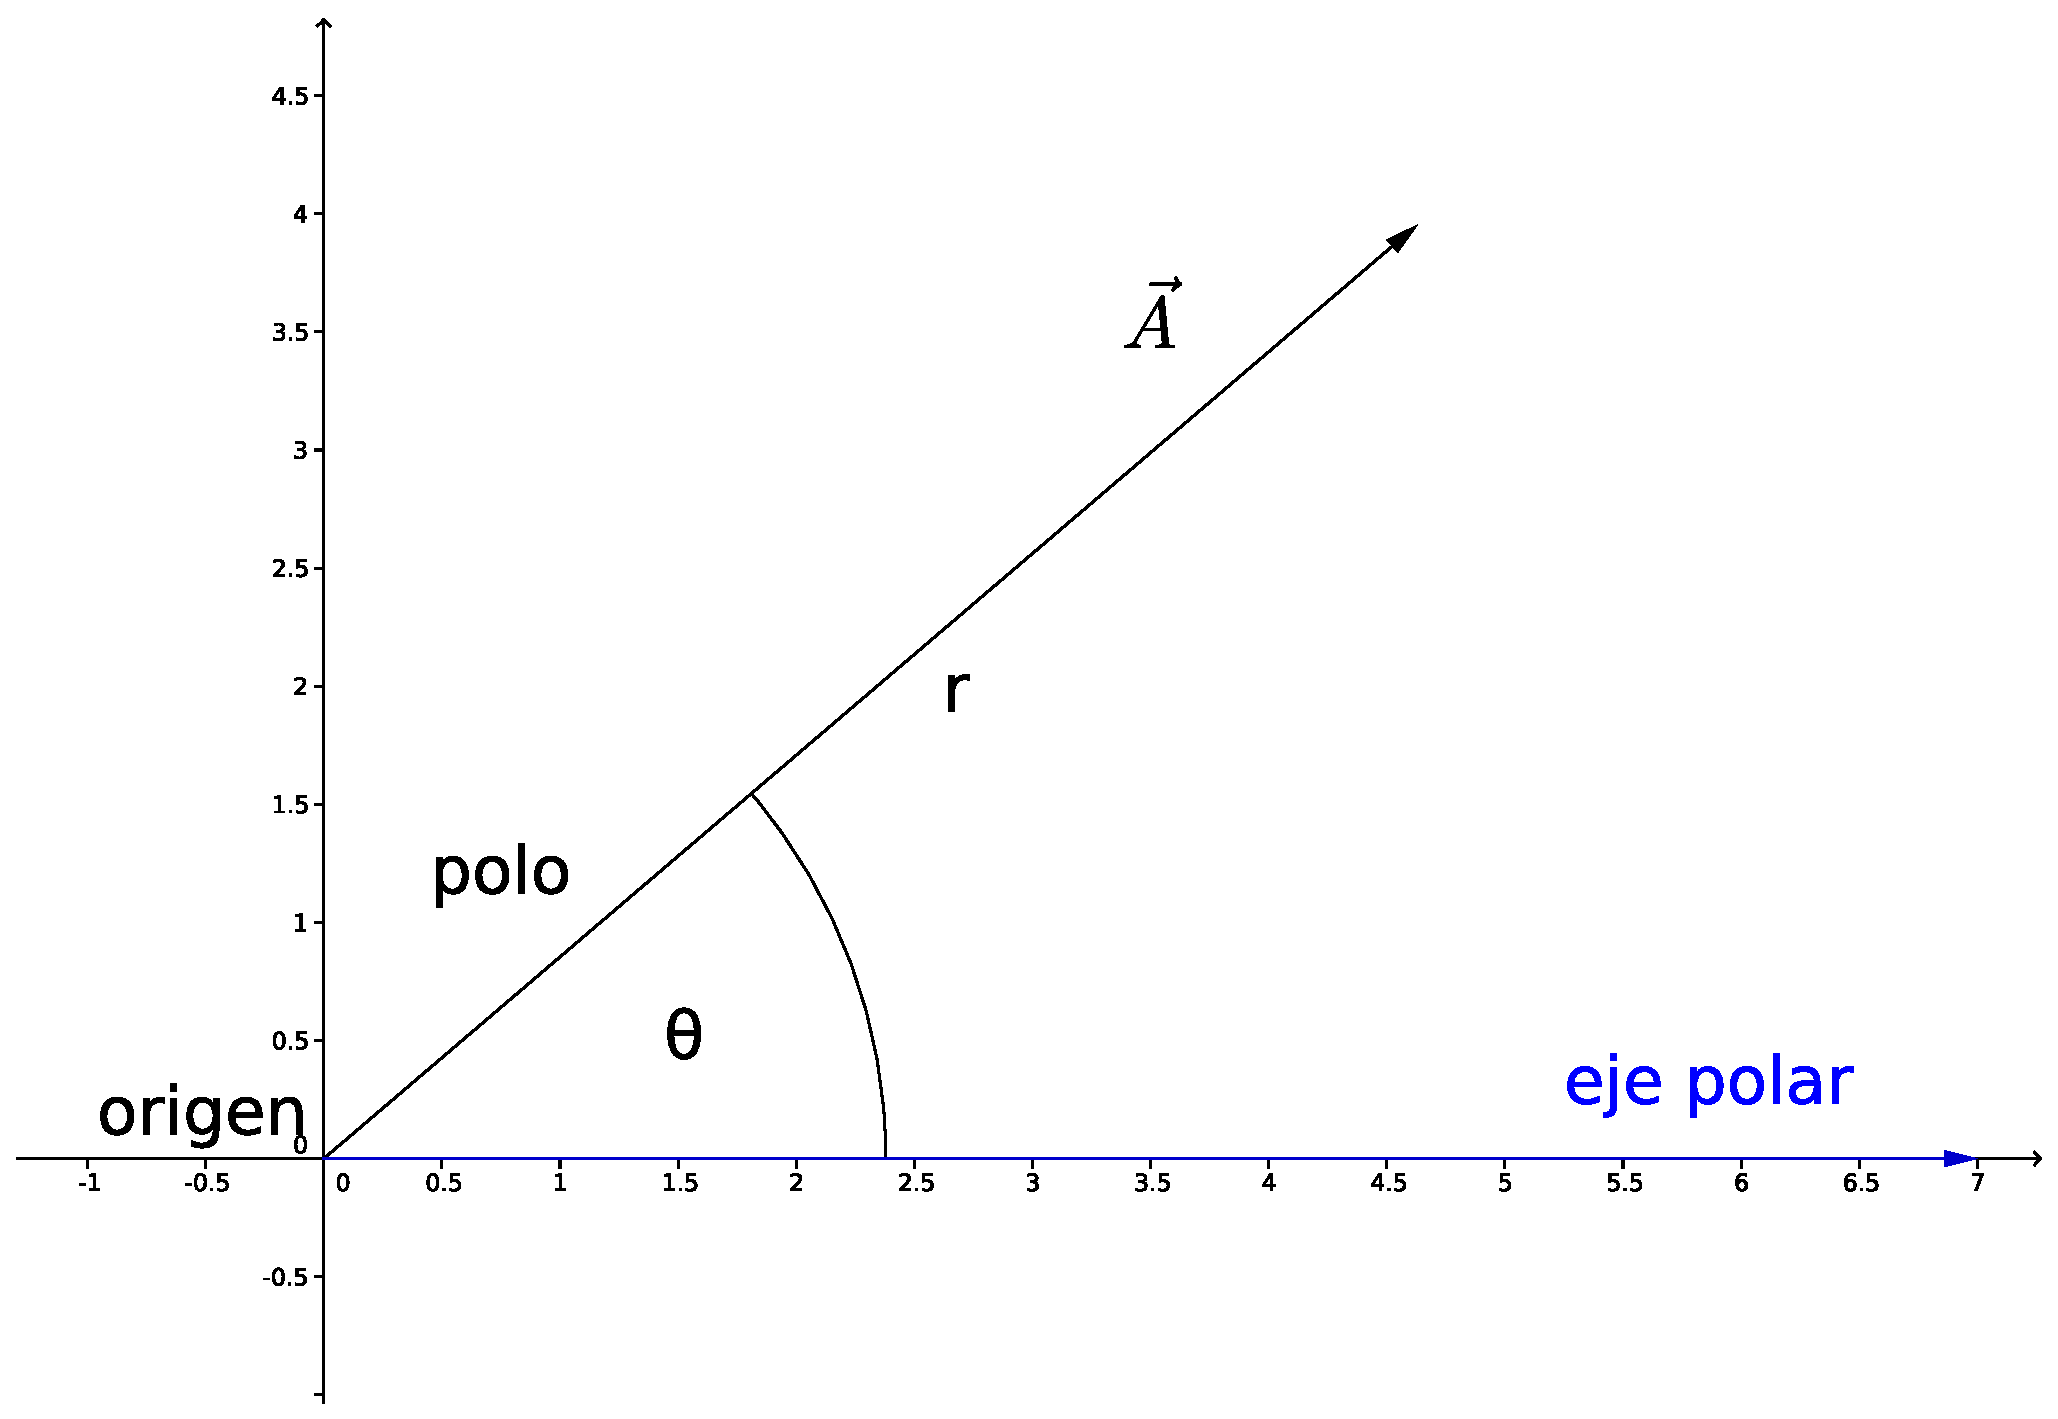
\includegraphics[width=0.7\textwidth]{images/vector_tres.eps}
  \caption{\small{Representación de las coordenadas polares del vector $\vec{A}$ en el plano cartesiano.}}
   \end{figure}

Los vectores usualmente también se los representa en función de su módulo y dirección:

\begin{equation}
 \vec{A} = (|\vec{A}|, \theta)
\end{equation}

\subsection{Representación en coordenadas geográficas:}

\begin{figure}
 \centering
 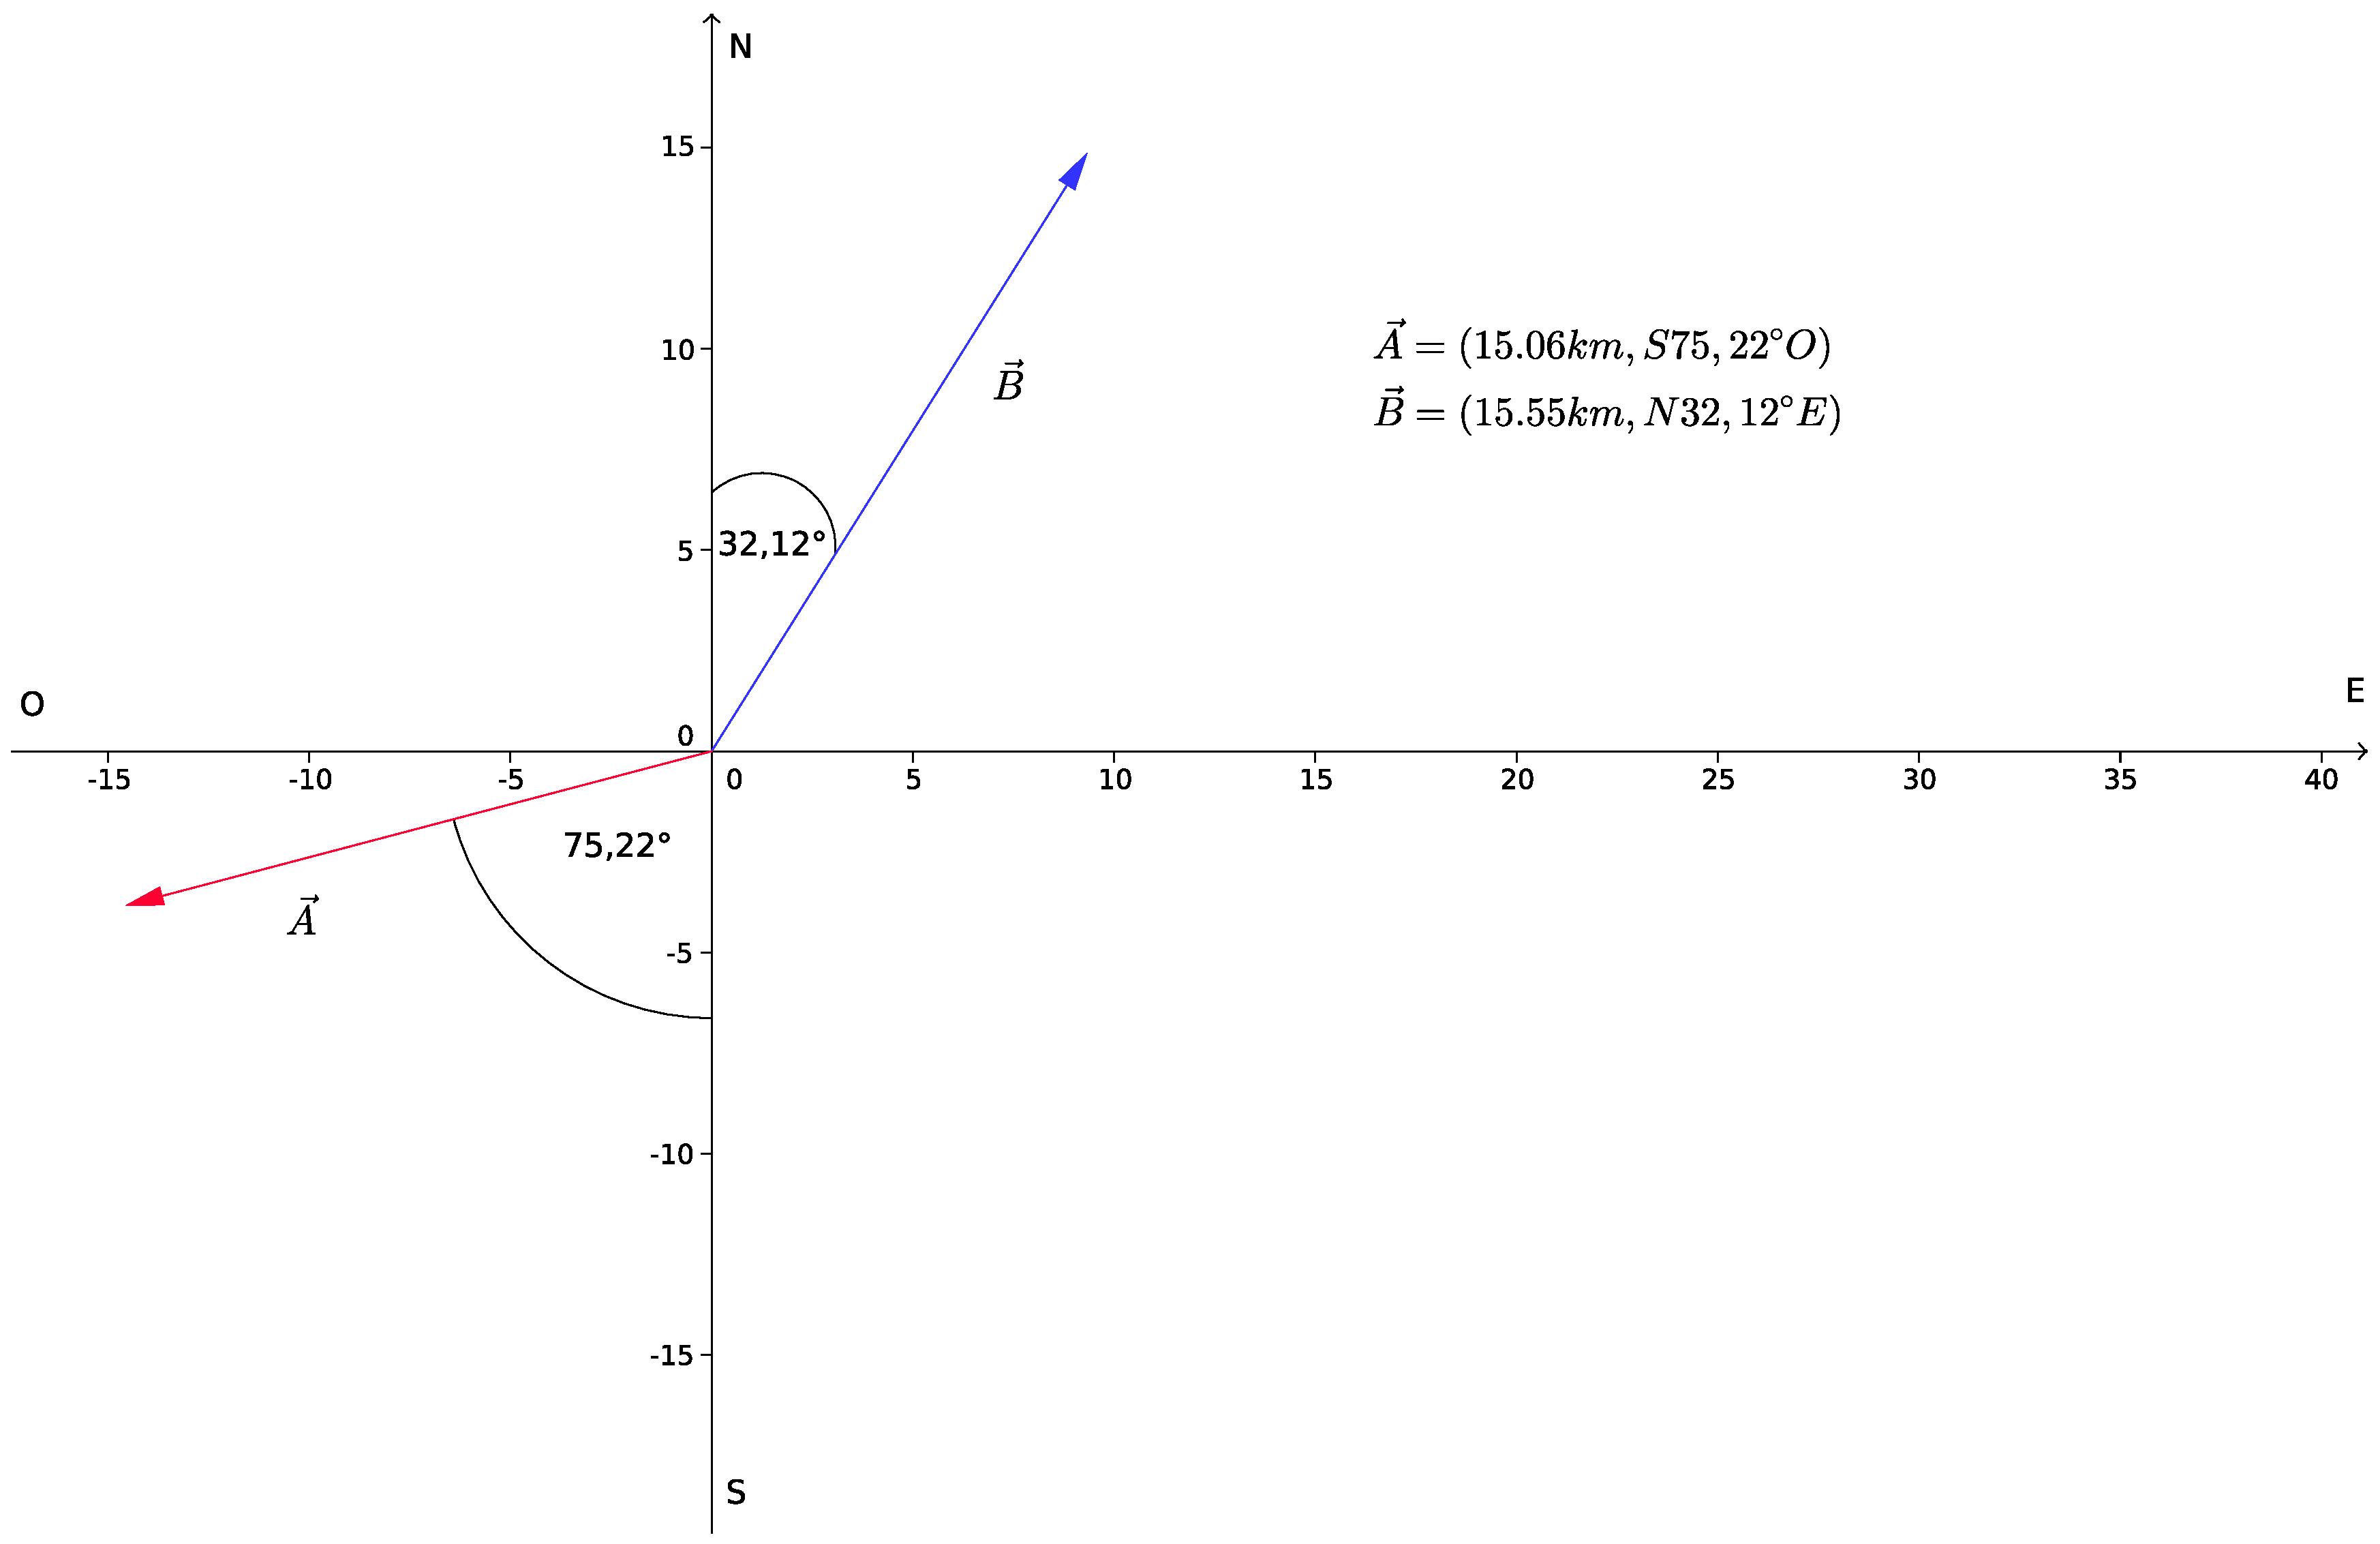
\includegraphics[width=1.1\textwidth]{images/vector_cuatro.eps}
   \caption{\small{Representación de las coordenadas geográficas de los vectores $\vec{A}$ y $B$.}}
\end{figure}

Un vector queda representado en coordenadas geográficas indicando primero su módulo, luego indicando a cual polo sea el 
Norte o el Sur al cual el vector está más cercano, posteriormente el ángulo desde ese eje hacia el vector y finalmente 
hacia que dirección sea Este o Oeste queda más cercana el vector.

\subsection{Suma y resta de vectores:}

Ya que las cantidades vectoriales poseen módulo y dirección, la suma de estas cantidades no sigue las reglas de la suma 
tradicional de los escalares.

\subsubsection{Método del paralelogramo:}

\begin{figure}
\centering
 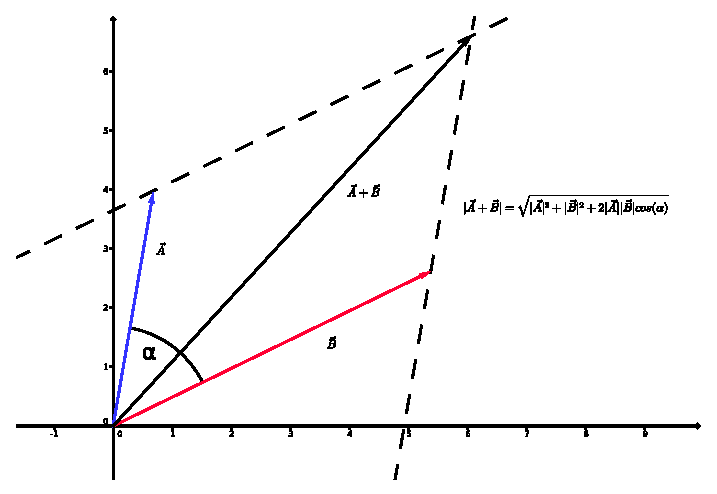
\includegraphics[scale=0.9]{images/vector_cinco.eps}
    \caption{\small{Representación de la suma entre dos vectores.}}
\end{figure}

El método del paralelogramo es un procedimiento gráfico sencillo que permite hallar la suma de dos vectores.

\begin{itemize}
 \item Primero se dibujan ambos vectores a escala, con el punto de aplicación común.
 \item Seguidamente, se completa un paralelogramo, dibujando dos segmentos paralelos a ellos.
 \item El vector suma resultante ($\vec{a} + \vec{b}$) será la diagonal del paralelogramo con origen común a los dos 
 vectores originales.
\end{itemize}

\subsubsection{Método cabeza - cola:}

\begin{figure}[H]
 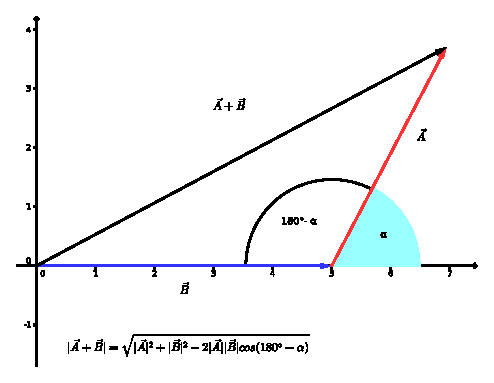
\includegraphics[scale=1.1]{images/vector_seis.eps}
    \caption{\small{Representación del método cabeza - cola.}}
 % suma-vectores-metodo-cabeza-cola.jpg: 410x261 px, 96dpi, 10.85x6.91 cm, bb=0 0 308 196
\end{figure}

Se trata de una variante del método del paralelogramo. Se desplaza el vector $\vec{b}$ paralelamente hasta el extremo 
del vector $\vec{a}$. El lado que completa el triángulo es el vector suma ($\vec{a} + \vec{b}$), cuyo inicio está en el 
extremo del primer vector $\vec{a}$ y su fin en el final del segundo vector sumando $\vec{b}$. 
    
\subsubsection{Método analítico:}     

A diferencia de los dos anteriores métodos, este se trata de un método analítico algebraico que no requiere de la 
realización del gráfico y por tanto es el más práctico y útil. Este método se trata de que primero los vectores a sumar 
deben estar expresados en sus coordenadas cartesianas y posteriormente se suman algebraicamente las componentes de los 
vectores en el eje x y así mismo en el eje y.

\begin{tcolorbox}
 Si $\vec{a} = a_x\vec{i}+a_y\vec{j}$ y $\vec{b} = b_x\vec{i}+a_y\vec{j}$, entonces el vector suma o resultante de los 
dos es: $\vec{c} =\vec{a}+\vec{b}$ tal que: $\vec{c} = (a_x + b_x)\vec{i} +(a_y+b_y)\vec{j}$. 
\end{tcolorbox}

\subsubsection{Propiedades de la suma:}

\textbf{Propiedad asociativa:}

\begin{equation}
 \vec{a} + (\vec{b} + \vec{c}) = (\vec{a} + \vec{b}) + \vec{c} = (\vec{a} + \vec{c}) +\vec{b} 
 \end{equation}

\textbf{Propiedad conmutativa:}
\begin{equation}
 \vec{a} + \vec{b} = \vec{b} + \vec{a}
\end{equation}

\textbf{Elemento opuesto:}

\begin{equation}
 \vec{a} + \vec{b} = \vec{0} \quad \text{si y solo si}\quad \vec{b} =-\vec{a} 
\end{equation}

\textbf{Elemento neutro:}

\begin{equation}
 \vec{a} + \vec{0} = \vec{a} 
\end{equation}

\subsection{Producto escalar o punto:}

\begin{figure}[H]
 \centering
 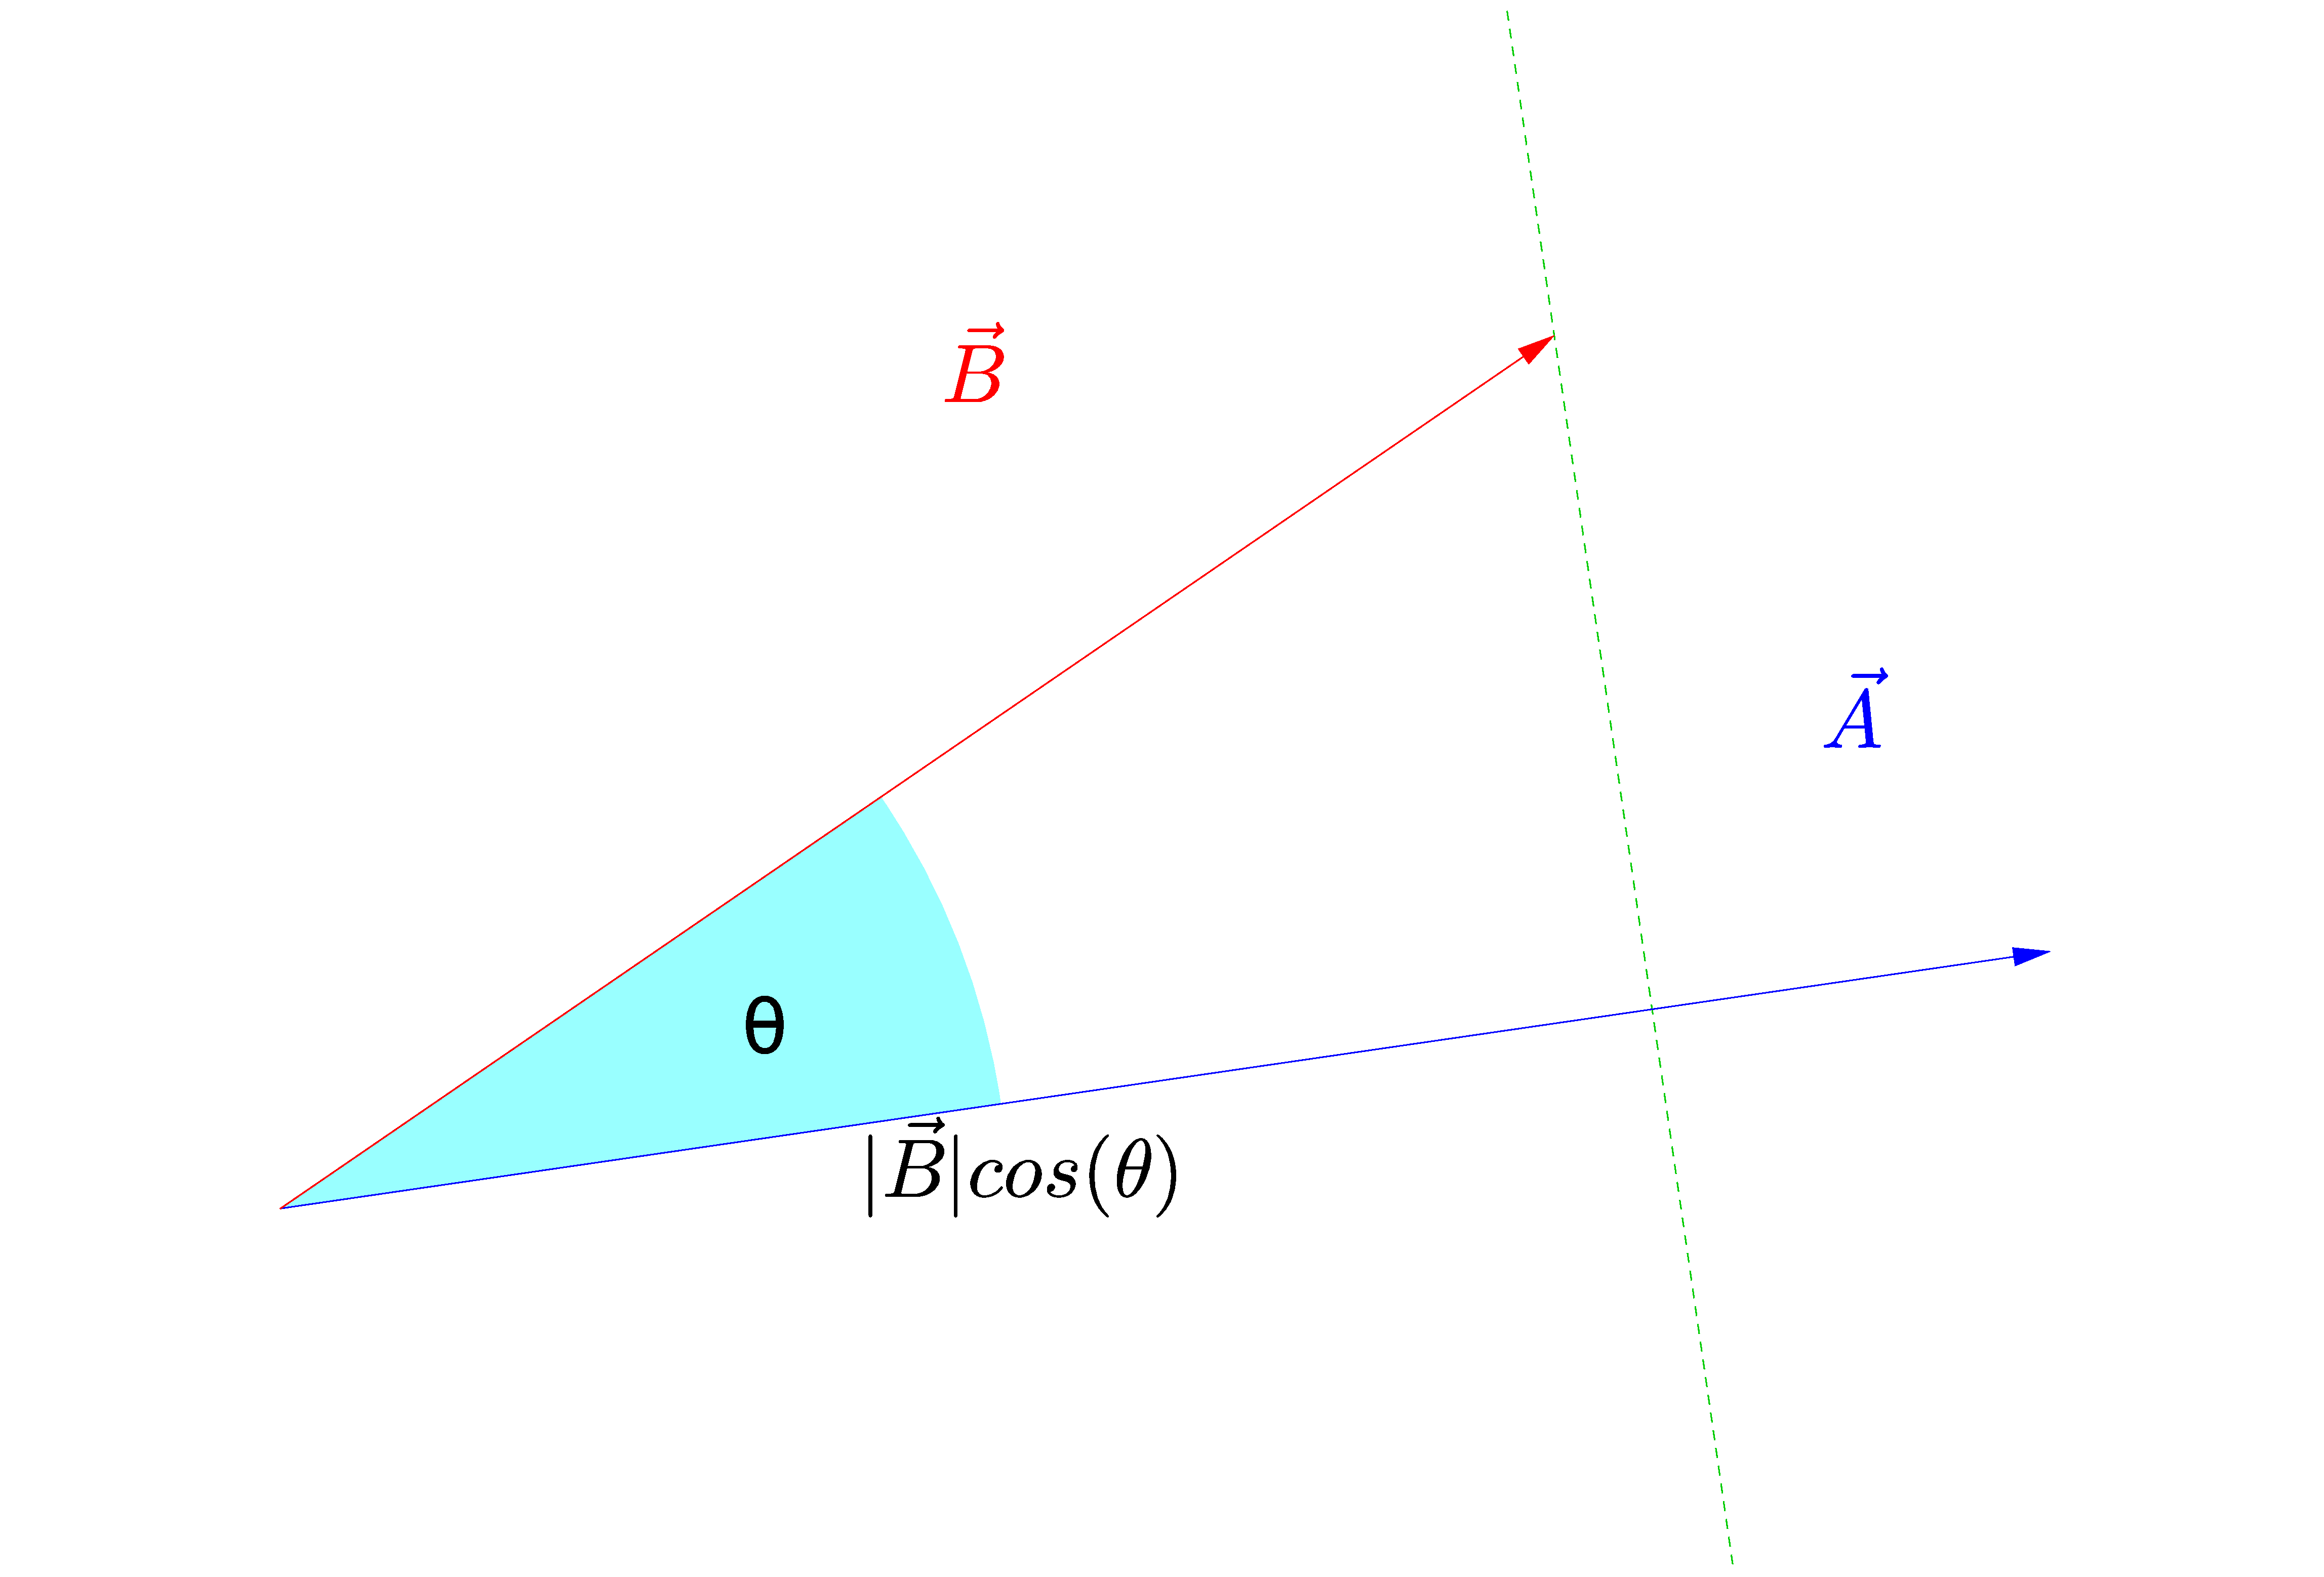
\includegraphics[width=0.7\textwidth]{images/vector_siete.eps}
 % productoescalar.png: 200x200 px, 72dpi, 7.06x7.06 cm, bb=0 0 200 200
 \caption{Ilustración geométrica del producto entre dos vectores.}
 \label{fig:escalar}
\end{figure}

Este producto se da entre dos vectores y su resultado es una cantidad escalar. Este operación se realiza de la 
siguiente manera:

\begin{tcolorbox}
Sean $\vec{a} =a_x\vec{i}+a_y\vec{j}$ y $\vec{b}=b_x\vec{i}+b_y\vec{j}$ dos vectores entonces el producto escalar 
entre ellos se define como $\vec{a}\cdot\vec{b}=|\vec{a}||\vec{b}|cos(\theta)= a_xb_x+a_yby$, donde $\theta$ es el 
ángulo formado entre los dos vectores.
\end{tcolorbox}

Así, es obvio que el producto escalar entre dos vectores que son perpendiculares es cero debido a que el ángulo entre 
ellos es de $90^\circ$.\\

Este producto tiene una interpretación geométrica que corresponde al área del paralelogramo formado entre los dos vectores.\\

A través del uso de este producto se puede calcular la proyección de un vector sobre otro de la siguiente manera:

\begin{tcolorbox}
La proyección de un vector $\vec{b}$ sobre otro vector $\vec{a}$ se define como: $\text{proj}_{\vec{a}}\vec{b} 
=|\vec{b}|cos(\theta)= \frac{\vec{a}\cdot\vec{b}}{|\vec{a}|}$.
\end{tcolorbox}

\subsection{Producto vectorial de vectores:}

\begin{figure}[H]
 \centering
 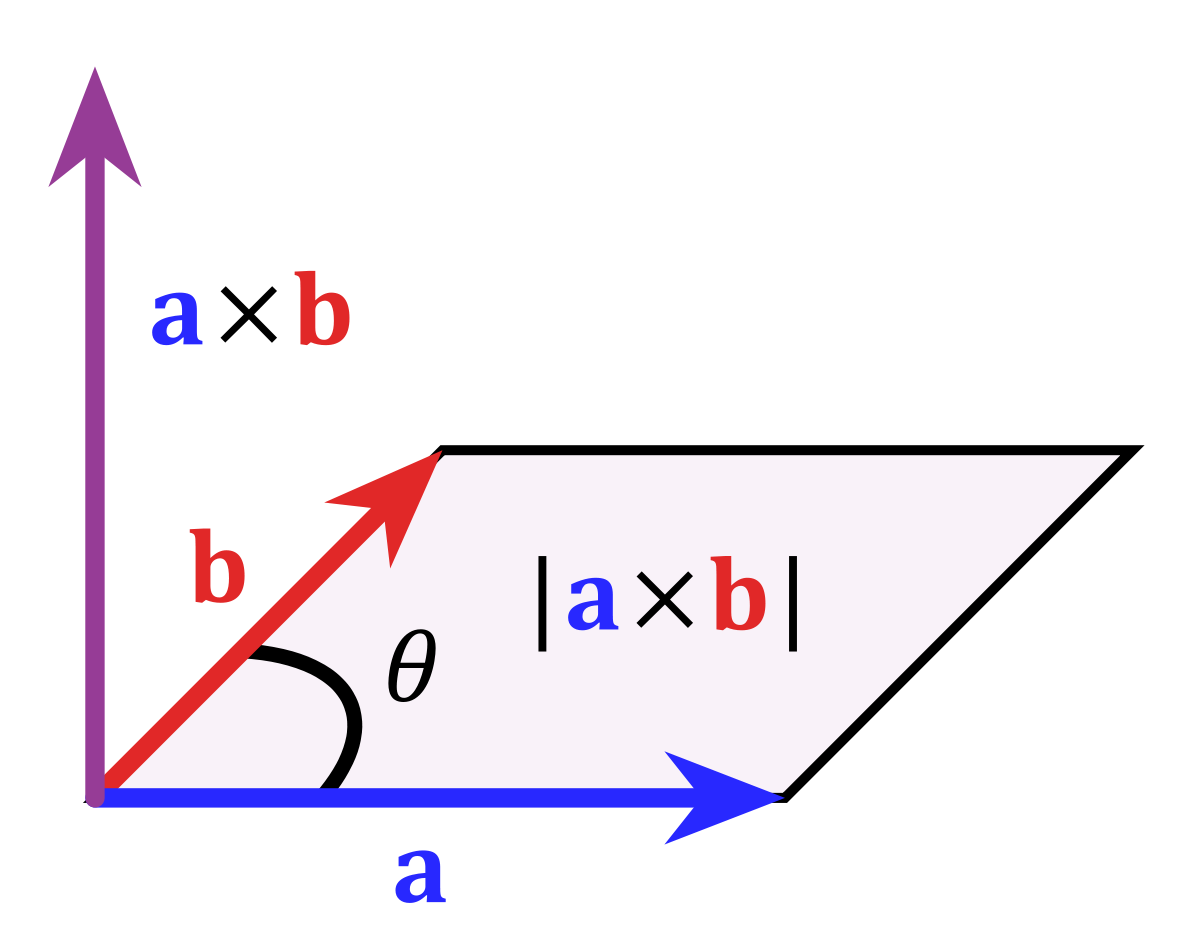
\includegraphics[scale=0.1]{images/1200px-Cross_product_parallelogram.png}
 % 1200px-Cross_product_parallelogram.svg.png: 1200x938 px, 72dpi, 42.33x33.09 cm, bb=0 0 1200 938
 \caption{Ilustración del producto vectorial entre vectores.}
 \label{fig:vectorial}
\end{figure}

Este producto se da entre dos vectores dando como resultado otro vector. Este producto se define de la siguiente manera:

\begin{tcolorbox}
 Sean $\vec{a} =a_x\vec{i}+a_y\vec{j}+a_z\vec{k}$ y $\vec{b}=b_x\vec{i}+b_y\vec{j}+b_z\vec{k}$ dos vectores entonces el 
 producto vectorial entre ellos se define como: 
\scriptsize{ 
 \[
\vec{a}\times\vec{b} =
\begin{vmatrix}
\vec{i} & \vec{j} & \vec{k} \\ 
a_x & a_y & a_z \\
b_x & b_y & b_z
\end{vmatrix} = (a_yb_z-b_ya_z)\vec{i}-(a_xb_z-a_zb_x)\vec{j}+(a_xb_y-b_xa_y)\vec{k}
\]}
\end{tcolorbox}

Siendo el vector $\vec{a}\times\vec{b}$ perpendicular a los vectores $\vec{a}$ y $\vec{b}$, y que cuyo módulo es:

\begin{equation}
 |\vec{a}\times\vec{b}|=|\vec{a}||\vec{b}|sen(\theta)
\end{equation}

Cabe resaltar que para este producto es necesario utilizar el eje coordenado espacial $z$ cuyo vector base en 
$\vec{k}$. En cuanto a la dirección del vector resultante está dada por la regla de la mano derecha. Por otro lado este 
producto da como resultado igual a cero si los vectores operandos son paralelos.

\begin{tcolorbox}
La dirección del vector $\vec{a}\times\vec{b}$ estaría definida por la dirección del pulgar, cerrando los demás dedos en torno al 
vector $\vec{a}$ primero y siguiendo con el vector $\vec{b}$.
\end{tcolorbox}

Así, cabe destacar que se cumple lo siguiente $\vec{a}\times\vec{b}=-\vec{b}\times\vec{a}$. También el módulo del producto 
vectorial de dos vectores equivale al área del paralelogramo construído en estos vectores.

\subsection{Problemas de vectores:}

\begin{enumerate}
 
 \item Calcular el vector unitario del vector $\vec{H} = 2\vec{i}+3\vec{j}$.
 
 \item Siendo el vector G = 3i – 5j, expresarlo en coordenadas polares y geográficas.
 
 \item Sean los vectores: A =(3,3), B=(-1,0) y C(2,2). Hallar la suma de esos vectores.
 
\item Sean los vectores: A =(3,3), B=(-1,0) y C(2,2). Hallar: 3A-4B+5C.

\item Que vector le debo restar al vector E =(8,7), para obtener el vector A =(2,3).
 
 \item Encuentre el módulo y dirección del vector $\vec{a}= \vec{i} - \vec{j}$.
 
 \item Encuentre el vector unitario del anterior problema.
 
 \item Hallar las coordenadas del punto C, sabiendo que B(2,2) es el punto medio de AC, A(3,1).
 
 \item Dos vectores forman entre sí un ángulo de 60°, si el valor de su resultante es de 156 unidades, y la magnitud de uno 
de los vectores componentes es de 100 unidades, ¿cuál será la magnitud del otro vector?
 
 \item Un alumno camina 50 m hacia el este, a continuación 30 m hacia el sur, después 20 m hacia el oeste, y finalmente, 10 m 
hacia el norte. Determina el vector desplazamiento desde el punto de partida hasta el punto de llegada. (incluyendo el ángulo que 
determina su dirección)
 
 \item Encuentre la suma de los vectores $\vec{c}=\vec{i}+\vec{j}$ y $\vec{d}=2\vec{i}-3\vec{d}$.
 
 \item Encuentre también la diferencia.
 
 \item Dado el vector $a =(3,-4)$, calcular el vector libre $b$ que tiene: la misma dirección y sentido que $a$ y módulo 
igual a la unidad.

\item Encuentre el producto escalar entre los siguientes vectores: $\vec{A} = 2\vec{i} + 3\vec{j}$ y $\vec{D} = 3\vec{i} - 
\vec{j}$.
 
 \item Exprese el siguiente vector en coordenadas cartesianas: c = (5, NE)
 
 \item Encuentre el vector unitario del vector que es opuesto al siguiente vector $\vec{S} =  10\vec{i}-7\vec{j}$.
 
 \item Encuentre el valor de t para el cual el siguiente vector resulta ser unitario: $\vec{v} = (t+1)\vec{i} +(t-1)\vec{j}$.

 
 \item Un vector hace un ángulo de $240^\circ$ en sentido antihorario con el eje de las abcisas y el valor de su componente 
en ese mismo eje es de 200 m, halle el vector unitario de ese vector.
 
 \item Encuentre el módulo del siguiente vector: $5\vec{d}-2\vec{c}$, donde $d=(34 m/s, 330^\circ)$ y $c = (54m/s, S20^\circ 
O)$.

\item Averigue si los vectores A = (-3,4) y B = (3,4) son perpendiculares entre si.
 
 \item Determina las coordenadas geográficas del siguiente vector: $\vec{R}=(23 m/s,N45^\circ E)$.
 
 \item Determina las coordenadas polares del siguiente vector: $\vec{T}=(7\vec{i}-4\vec{j})kgf$.
 
 \item Determina las coordenadas cartesianas del vector: $\vec{h}=(13,330^\circ)$.
 
 \item Encuentre el módulo del siguiente vector: 5d−2c, donde d = (34m/s, $330^\circ$ ) y c = (54m/s,
S$20^\circ$ O).

 \item Calcula el producto escalar entre $\vec{a}=6\vec{i}-7\vec{j}$ y $\vec{b}=-4\vec{i}+10\vec{j}$.

\item Determina si $\vec{a} = 12\vec{i}-13\vec{j}$ es perpendicular al vector $\vec{b}=4\vec{i}-3\vec{j}$.

\item Determine la proyección del vector $\vec{r} = (23 km, N40^\circ O)$ sobre el vector $\vec{q}=(40km,230^\circ)$.

\item Determine el área del paralelogramo formado por los vectores $\vec{u}=(1,1)$ y $\vec{v}=(1,-1)$.

\item Siendo los vectores $\vec{a} = (2,3)$, $\vec{b} = (-3,5)$ y $\vec{c} = (4,-1)$, calcular lo siguiente: 
$3\vec{a}\cdot\frac{1}{2}(\vec{c}+\vec{b})-7\vec{b}\cdot\vec{c}+5\vec{a}\cdot(\vec{c}-\vec{a})$ 

\item Dado los vectores $\vec{v} = 3\vec{i}-\vec{j}+4\vec{k}$ y $\vec{w}=-\vec{i}+3\vec{j}+5\vec{k}$, calcule lo 
siguiente: $\frac{1}{2}\vec{v}\times\vec{w}$.

\item Sabiendo que $\vec{A} = (m - 1) \vec{i} + (2 m + 3) \vec{j}$ y $\vec{B} = (m - 2) \vec{i} + (2 m - 19) \vec{j}$. 
Encuentre el número real m para que se cumpla que $3 \vec{A} + \vec{B} = 0$.

\item Halle el vector unitario del siguiente vector: A = (3,4), y luego encuentre su opuesto.

\item ¿Qué vector le debo restar al vector $\vec{v} = (2,4)$ para tener que el resultado sea el doble del vector $\vec{w} = 
(-2,3)$?.

\item Un automóvil recorre 3 km hacia el Norte y luego 5 km hacia el Norte $40^\circ$ Este, representar estos desplazamientos y 
hallar el desplazamiento resultante gráfica y analíticamente.

\item Calcula el valor de k sabiendo que el módulo del vector $\vec{v}$= (k, 3) es 5.

\item Dos vectores tienen como longitud 9 y 6 cm, formando entre sí ángulos de $180^\circ$, $60^\circ$, $150^\circ$, $0^\circ$. 
Halla gráficamente y analíticamente la magnitud del vector resultante y el ángulo que determina su dirección y sentido.

\item Dos vectores forman entre sí un ángulo de $60^\circ$, si el valor de su resultante es de 156 unidades, y la magnitud de uno 
de los vectores componentes es de 100 unidades, ¿cuál será la magnitud del otro vector?

\item Un alumno camina 50 m hacia el este, a continuación 30 m hacia el sur, después 20 m hacia el oeste, y finalmente, 10 m 
hacia el norte. Determina el vector desplazamiento desde el punto de partida hasta el punto de llegada. (incluyendo el ángulo que 
determina su dirección)

\item Una mosca se para en la pared de un cuarto. La esquina inferior izquierda de la pared se selecciona como el origen de un 
sistema de coordenadas cartesianas en dos dimensiones. Si la mosca está parada en el punto que tiene coordenadas (2, 1) m, (a) 
¿qué tan lejos está de la esquina del cuarto?, (b) ¿Cuál es su posición en coordenadas polares?

\end{enumerate}
